\documentclass[../Main.tex]{subfiles}

\begin{document}
In three dimensions, the Time Independent Schr\"odinger Equation is:
\begin{equation}
    -\frac{\hbar^2}{2m} \nabla^2 \chi(\vec{x}) + U(\vec{x}) \chi(\vec{x}) = E \chi(\vec{x})
    \label{eqnTISE3D}
\end{equation}
\section{Reminder of Coordinate Systems}
We will use Cartesian coordinates $(x, y, z)$ and Spherical coordinates $(r, \theta, \phi)$. We denote the angle from the positive $z$-axis by $\theta$.
In these coordinate systems, the Laplacian is:
\begin{align*}
    \text{Cartesian: } \nabla^2&= \frac{\partial^{2}}{\partial x^{2}} + \frac{\partial^{2}}{\partial y^{2}} + \frac{\partial^{2}}{\partial z^{2}} \\
    \text{Spherical: } \nabla^2 &= \frac{1}{r^2} \frac{\partial}{\partial r}\left(r^2\frac{\partial}{\partial r}\right) + \frac{1}{r^2 \sin{\theta}} \frac{\partial }{\partial \theta}\left(\sin{\theta} \frac{\partial}{\partial \theta}\right)\\
    &\qquad+ \frac{1}{r^2 \sin^2{\theta}}\frac{\partial^{2}}{\partial \phi^{2}}
\end{align*}
For the spherical polars expression, we can simplify the term in $r$:
\begin{equation*}
    \nabla f = \frac{1}{r} \frac{\partial^2}{\partial r^2} (rf) + \frac{1}{r^2 \sin^2{\theta}}\left[\sin{\theta} \frac{\partial}{\partial \theta}\left(\sin{\theta} \frac{\partial f}{\partial \theta}\right) + \frac{\partial^{2}f}{\partial \phi^{2}}\right] 
\end{equation*}
Recall the different volume integrals:
\begin{align*}
    \text{Cartesian: }&\int_{\R^3} dV = \int_{x = -\infty}^{\infty} \int_{y = -\infty}^{\infty} \int_{z = -\infty}^{\infty} f(x, y, z) dz~dy~dx \\
    \text{Spherical: }&\int_{\R^3} dV = \int_{r = 0}^{\infty} \int_{\phi = 0}^{2\pi} \int_{\theta = 0}^{\pi} f(r, \phi, \theta) r^2 \sin{\theta}~d\theta~d\phi~dr \\
\end{align*}
We will consider only spherical potentials $U(\vec{x}) = U(r)$.

\section{Angular Momentum}
\subsection{Definition and Commutativity}
In classical mechanics, we used the constant angular momentum to simplify 3-dimensional problems with a central potential into 2-dimensional ones. We will also define the angular momentum in Quantum Mechanics:
\begin{definition}{Angular momentum}
    The \underline{angular momentum} in Quantum mechanics is an operator:
    \begin{equation}
        \opvec{L} = \opvec{x} \times \opvec{p} = -i\hbar \opvec{x} \times \nabla
        \label{eqnQAngMomentum}
    \end{equation}
\end{definition}
We can show (an indeed do in Ex3) that $\opvec{L}$ is Hermitian, and so are its components $\hat{L}_i$.
\begin{proposition}
    For distinct $i, j \in \{1, 2, 3\}$, the commutator of different elements of the angular momentum operator is:
    \begin{equation}
        [\hat{L}_i, \hat{L}_j] = i \hbar \epsilon_{ijk} \hat{L}_k
        \label{eqnAngMomCmmt}
    \end{equation}
    \label{propAngMomCmmt}
\end{proposition}
\begin{remark}
    The commutator is non-zero, which tells us that we cannot measure the angular momentum to arbitrary precision, because if we measure one element to arbitrary precision then we have a lower bound on the precision of the other two elements' measurements.
\end{remark}
\begin{proof}
    The proof is simply by multiplying the commutator out. First we need the commutator of $\hat{x}_i$ and $\hat{p}_j$:
    \begin{align*}
        [\hat{x}_i, \hat{p}_j] &= \hat{x}_i \hat{p}_j - \hat{p}_j \hat{x}_i \\
        &= -i\hbar \left(x_i \frac{\partial}{\partial x_j} - \frac{\partial}{\partial x_j} (x_i \cdot)\right) \\
        &= -i\hbar \left(x_i \frac{\partial}{\partial x_j} - x_i\frac{\partial}{\partial x_j} - \left(\frac{\partial x_i}{\partial x_j} \times \cdot \right)\right) \\
        &= -i\hbar \left(- \delta_{ij} \hat{I}\right) \\
        &= i\hbar \delta_{ij} \hat{I}
    \end{align*}
    Now we can use this to find $\hat{L}_i \hat{L}_j$:
    \begin{align*}
        \hat{L}_i \hat{L}_j&= \epsilon_{ikl} \hat{x}_k \hat{p}_l \epsilon_{jmn} \hat{x}_m \hat{p}_n \\
        &= \epsilon_{ikl} \epsilon_{jmn} \hat{x}_k \hat{p}_l \hat{x}_m \hat{p}_n \\
        &= \epsilon_{ikl} \epsilon_{jmn} \hat{x}_k (\hat{x}_m \hat{p}_l - [\hat{p}_l, \hat{x}_m]) \hat{p}_n \\
        &= \epsilon_{ikl} \epsilon_{jmn} \hat{x}_k (\hat{x}_m \hat{p}_l - i\hbar \delta_{lm} \hat{I}) \hat{p}_n \\
        &= \epsilon_{ikl} \epsilon_{jmn} \hat{x}_k \hat{x}_m \hat{p}_l \hat{p}_n - i \hbar\epsilon_{ikl} \epsilon_{jln} \hat{x}_k \hat{p}_n \\
        &= \epsilon_{ikl} \epsilon_{jmn} \hat{x}_k \hat{x}_m \hat{p}_l \hat{p}_n - i \hbar (\delta_{in} \delta_{kj} - \delta_{ij} \delta_{kn}) \hat{x}_k \hat{p}_n \\ 
        &= \epsilon_{ikl} \epsilon_{jmn} \hat{x}_k \hat{x}_m \hat{p}_l \hat{p}_n - i \hbar \hat{x}_j \hat{p}_i
    \end{align*}
    Then similarly, $\hat{L}_j \hat{L}_i = \epsilon_{jkl} \epsilon_{imn} \hat{x}_k \hat{x}_m \hat{p}_l \hat{p}_n - i \hbar \hat{x}_i \hat{p}_j$. Re-label the indices to match with the previous expression:
    \begin{align*}
        \hat{L}_j \hat{L}_i &= \epsilon_{jmn} \epsilon_{ikl} \hat{x}_m \hat{x}_k \hat{p}_n \hat{p}_l - i \hbar \hat{x}_i \hat{p}_j \\
        \hat{L}_j \hat{L}_i &= \epsilon_{jmn} \epsilon_{ikl} \hat{x}_k \hat{x}_m \hat{p}_l \hat{p}_n - i \hbar \hat{x}_i \hat{p}_j  \text{ by commutativity}
    \end{align*}
    which has the same first part as $\hat{L}_i \hat{L}_j$.

    Now find the commutator we want:
    \begin{align}
        [\hat{L}_i, \hat{L}_j] &= -i\hbar(\hat{x}_j \hat{p}_i - \hat{x}_i \hat{p}_j) \nonumber\\
        &= i\hbar(\hat{x}_i \hat{p}_j - \hat{x}_j \hat{p}_i) \label{eqnAngMomCmmt2}
    \end{align}
    and, by expanding out the $\epsilon_{ijk}$ in equation~\ref{eqnAngMomCmmt} in terms of index notation, we find that this is indeed the required result.
\end{proof}
\begin{remark}
    Equation~\ref{eqnAngMomCmmt2} gives an interesting alternate form to the commutator.
\end{remark}
\begin{definition}{Total angular momentum}
    The \underline{total angular momentum} operator is:
    \begin{equation}
        \hat{L}^2 = \hat{L}_1^2 + \hat{L}_2^2 + \hat{L}_3^2 = |\opvec{L}|^2
        \label{eqnTotAngMomentum}
    \end{equation}
\end{definition}
We can prove that the commutator is:
\begin{equation*}
    [\hat{L}^2, \hat{L}_i] = 0
\end{equation*}
This tells us that we can find the magnitude of $\opvec{L}$ and one of its components with arbitrary precision. We generally find the $z$-component of the angular momentum and its magnitude. This is equivalent to simultaneously diagonalising the two operators.
\subsection{Eigenfunctions of Angular Momentum}
\label{secSphericalHarmonics}
To find the joint set of eigenfunctions of $\hat{L}^2$ and $\hat{L}_3$, we write $\opvec{L}$ in spherical coordinates. This results in:
\begin{align*}
    \hat{L}_3 &= -i \hbar \frac{\partial}{\partial \phi} \\
    \hat{L}^2 &= -\frac{\hbar^2}{\sin^2{\theta}} \left[\sin{\theta} \frac{\partial}{\partial \theta}\left(\sin{\theta} \frac{\partial}{\partial \theta}\right) + \frac{\partial^{2}}{\partial \phi^{2}}\right]
\end{align*}
Then we find $Y(\theta, \phi)$, the joint eigenfunctions of these operators.
The equations for $Y$ are:
\begin{gather}
    -i\hbar \frac{\partial }{\partial \phi} Y(\theta, \phi) = \mu Y(\theta, \phi) \label{eqnAngMomEFunc1} \\
    -\frac{\hbar^2}{\sin^2{\theta}} \left[\sin{\theta} \frac{\partial}{\partial \theta}\left(\sin{\theta} \frac{\partial}{\partial \theta}\right) + \frac{\partial^{2}}{\partial \phi^{2}}\right] Y(\theta, \phi) = \lambda Y(\theta, \phi) \label{eqnAngMomEFunc2}
\end{gather}
Now we can look for separable solutions:
\begin{equation*}
    Y(\theta, \phi) = \Theta(\theta) \Phi(\phi)
\end{equation*}
Substituting this into equation~\ref{eqnAngMomEFunc1},
\begin{align*}
    -i \hbar \Phi'(\phi) \Theta(\theta) &= \mu \Phi(\phi) \Theta(\theta) \\
    \Phi'(\phi) &= \frac{i\mu}{\hbar} \Phi(\phi) \\
    \therefore \Phi(\phi) &= e^{\frac{i\mu}{\hbar} \phi}
\end{align*}
Now we note that the wavefunction $Y$ must be single-valued on $\R^3$, so we need invariance under $\phi \mapsto \phi + 2\pi$. Therefore, $\frac{\mu}{\hbar}$ must be an integer (quantisation). Re-label such that $m = \frac{\mu}{\hbar}$, so that $m$ is an integer and $\Phi(\phi) = e^{im\phi}$.

Now we can solve for $\Theta$. Using the separable solution in equation~\ref{eqnAngMomEFunc2}:
\begin{align}
    -\frac{\hbar^2}{\sin^2{\theta}}&\left[\sin{\theta} \frac{\partial}{\partial \theta}\left(\sin{\theta} \Theta'(\theta)\right)\Phi(\phi) + \Theta(\theta)\Phi''(\phi)\right] = \lambda \Theta(\theta) \Phi(\phi)\nonumber \\
    &= -\frac{\hbar^2}{\sin{\theta}} \frac{\partial }{\partial \theta} \left(\sin(\theta) \Theta'(\theta)\right) \Phi(\phi) +\frac{m^2 \hbar^2}{\sin^2{\theta}} \Phi(\phi) \Theta(\theta)
\end{align}
by substituting in $\Phi(\phi)$. Then divide through by $-\hbar^2 \Phi(\phi)$:
\begin{equation}
    \frac{1}{\sin{\theta}} \frac{\partial }{\partial \theta} \left(\sin(\theta) \Theta'(\theta)\right) -\frac{m^2}{\sin^2{\theta}} \Theta(\theta) = -\frac{\lambda}{\hbar^2} \Theta(\theta)
    \label{eqnAssocLegendre}
\end{equation}
This is similar to the Legendre equation from IB Methods. In fact, equation~\ref{eqnAssocLegendre} is the \textit{associated Legendre Equation}. Its solutions are the \textit{associated Legendre functions}:
\begin{align*}
    \Theta(\theta) &= P_{l, m} (\cos(\theta)) \\
    &= (\sin{\theta})^{|m|} \frac{d^{|m|}}{d(\cos(\theta))^{|m|}} P_l(\cos(\theta))
\end{align*}
where the $P_l(\cos(\theta))$ are the normal Legendre Polynomials.

Note that, if $|m| > l$, we have that $y(\theta) = 0$ because these polynomials have degree $l$ so taking too many derivatives means that the output is zero. This gives us a bound on $m$ in terms of $l$:
\begin{equation*}
    -l \leq m \leq l
\end{equation*}
Then the eigenvalues of $\hat{L}^2$ are given by:
\begin{equation*}
    \lambda = \hbar^2 l(l+1)
\end{equation*}
Putting everything together:
\begin{align*}
    Y_{l,m}(\theta, \phi) &= P_{l, m}(\cos(\theta)) e^{i m \phi} \\
    \hat{L}^2 Y_{l, m}(\theta, \phi) &= \hbar^2 l(l+1)Y_{l, m}(\theta, \phi) \\
    \hat{L}_3 Y_{l, m}(\theta, \phi) &= \hbar mY_{l, m}(\theta, \phi)
\end{align*}
The functions $Y_{l, m}$ are called \underline{spherical harmonics}.

The parameters $l, m$ are quantum numbers that characterise the total angular momentum ($l$), and the $z$ component of angular momentum ($m$, the \underline{azimuthal number}).

The first few states are:
\begin{align*}
    Y_{0, 0}(\theta, \phi) &= \frac{1}{\sqrt{4\pi}} \\
    Y_{1, 0}(\theta, \phi) &= \sqrt{\frac{3}{4\pi}} \cos(\theta) \\
    Y_{1, \pm 1}(\theta, \phi) &= \mp \sqrt{\frac{3}{8\pi}} \sin(\theta) e^{\pm \phi} \\
\end{align*}
Then like all eigenfunctions, we have an orthogonality relation:
\begin{equation*}
    \inn{Y_{l, m}}{Y_{l', m'}} = \delta_{ll'} \delta_{mm'}
\end{equation*}
\section{Spherically Symmetric Potential}
In spherical coordinates, the Laplacian is:
\begin{equation*}
    \nabla^2 = \frac{1}{r^2} \frac{\partial}{\partial r}\left(r^2\frac{\partial}{\partial r}\right) + \frac{1}{r^2 \sin{\theta}} \frac{\partial }{\partial \theta}\left(\sin{\theta} \frac{\partial}{\partial \theta}\right) + \frac{1}{r^2 \sin^2 \theta} \frac{\partial^{2}}{\partial \phi^{2}}
\end{equation*}
Then looking at the definition of $\hat{L}^2$, we observe:
\begin{equation*}
    -\hbar^2 \nabla^2 = \frac{\hbar^2}{r^2} \frac{\partial}{\partial r}\left(r^2\frac{\partial}{\partial r}\right) + \frac{\hat{L}^2}{r^2}
\end{equation*}
Then the Hamiltonian operator is:
\begin{equation}
    \hat{H} = -\frac{\hbar^2}{2mr^2} \frac{\partial}{\partial r}\left(r^2\frac{\partial}{\partial r}\right) + \frac{\hat{L}^2}{2mr^2} + U(\vec{x})
    \label{eqnHamiltonianAngMom}
\end{equation}
\begin{proposition}
    For a spherically symmetric potential $U(\vec{x}) = U(r)$,
    \begin{equation*}
        [\hat{H}, \hat{L}^2] = 0, \qquad [\hat{H}, \hat{L}_i] = 0
    \end{equation*}
    \label{propHamiltonianCommutes}
\end{proposition}
\begin{proof}
    We need to look at the following commutators:
    \begin{align*}
        [\hat{L}_i, \hat{x}_j]&= [\epsilon_{imn} \hat{x}_m \hat{p}_n, \hat{x}_j] \\
        &= \epsilon_{imn} \left(\hat{x}_m [\hat{p}_n, \hat{x}_j] + [\hat{x}_m, \hat{x}_j] \hat{p}_n\right) \\
        &= \epsilon_{imn} \left(\hat{x}_m [\hat{p}_n, \hat{x}_j] + 0\right)
    \end{align*}
    Note also that we found $[\hat{p}_n, \hat{x}_j] = -i\hbar \delta_{nj}$:
    \begin{align*}
        [\hat{L}_i, \hat{x}_j]&= -i \hbar\epsilon_{imj} \hat{x}_m \\
        &= i \hbar \epsilon_{ijk} \hat{x}_k
    \end{align*}
    Similarly we find:
    \begin{align*}
        [\hat{L}_i, \hat{x}_j^2] &= [\hat{L}_i, \hat{x}_j]\hat{x}_j + \hat{x}_j [\hat{L}_i, \hat{x}_j] \\
        &= i \hbar \epsilon_{ijk} \left(\hat{x}_k \hat{x}_j + \hat{x}_j \hat{x}_k\right) \\
        &= 0
    \end{align*}
    because this is a product of an antisymmetric tensor with a symmetric tensor.
    Therefore, since $U(r)$ is a function containing only $\hat{x}_i^2$,
    \begin{equation*}
        [\hat{L}_i, U(r)] = 0
    \end{equation*}
\end{proof}
\begin{remark}
    We can analogously find:
    \begin{align*}
        [\hat{L}_i, \hat{P}_j] &= i \epsilon_{ijk} \hat{p}_k \\
        [\hat{L}_i, \hat{P}_j^2] &= 0 \\
        [\hat{L}_i, \hat{p}^2] &= [\hat{L}_i, \hat{P}_1^2 + \hat{p}_2^2 + \hat{p}_3^2] = 0 \\
    \end{align*}
    and note also that $\hat{p}^2 = -\hbar^2 \nabla^2$. This tells us that:
    \begin{align*}
        [\hat{H}, \hat{L}^2] &= 0 \\
        [\hat{H}, \hat{L}_i] &= 0
    \end{align*}
\end{remark}
In particular we find that $\{\hat{H}, \hat{L}^2, \hat{L}_i\}$ is a set of \underline{mutually commuting}\\\underline{operators}. This means we can find joint eigenstates of these three operators, that form a basis of $\hilb$.

Further, this means that the eigenvalues $E, |\vec{L}|^2, L_z$ can be simultaneously measured, with arbitrary precision.

It is very hard to prove, but is true, that this set of operators is \underline{maximal}. That is, we cannot construct another nontrivial operator that commutes with elements in this set.

We will start by looking for the solutions of the TISE such that $\chi(r)$ satisfies $\hat{L}^2 \chi(r) = 0$.

Substituting this in:
\begin{align}
    \nabla^2 \chi(r) &= \frac{1}{r} \frac{d^{2}}{d x^{2}}(r\chi(r)) \nonumber \\
    \implies -\frac{\hbar^2}{2m} &\left(\frac{d^{2}\chi(r)}{dr^{2}}+ \frac{2}{r} \frac{d\chi(r)}{dr}\right) + U(r) \chi(r) = E\chi(r) \label{eqnTISESpherical}
\end{align}
We must also consider the normalisation conditions for $\chi$. These are slightly more complex in 3 dimensions. We need:
\begin{align*}
    1 &= \int_{\R^3} |\chi(r)|^2 dV \\
    &= 4\pi \int_{0}^\infty |\chi(r)|^2 r^2 dr
\end{align*}
Then for this to hold, require that the eigenfunction $\chi(r)$ goes to $0$ as $r \to \infty$ sufficiently fast. This we have used often for 1-dimensional solutions.

However, we also require that $\chi$ is well-behaved at $0$. We can be fairly relaxed with this condition, because we are multiplying by $r$ and then squaring, so we can permit, at worst, solutions containing terms like $\frac{1}{r}$.

To solve equation~\ref{eqnTISESpherical}, we define $\sigma(r) = r \chi(r)$. Then:
\begin{equation}
    -\frac{\hbar^2}{2m} \frac{d^{2}\sigma(r)}{dr^{2}} + U(r) \sigma(r) = E\sigma(r)
    \label{eqnTISESpherical2}
\end{equation}
This looks very familiar! However, we only define it on $r \geq 0$, and the normalisation condition is instead:
\begin{equation*}
    \int_{0}^{\infty} |\sigma(r)|^2 dr = \frac{1}{4\pi}
\end{equation*}
To understand our boundary conditions, we have to exclude an important case.
\begin{proposition}
    If $\sigma(r)$, as above defined, tends to a non-zero constant $a$ as $r \to 0$, the Hamiltonian operator $\hat{H}$ is not Hermitian.
    \label{propSigmaConstNoHerm}
\end{proposition}
\begin{proof}
    For $\hat{H}$ to be Hermitian we want $\inn{\phi}{\hat{H}\chi} = \inn{\hat{H} \phi}{\chi}$ for all $\phi, \chi \in \hilb$.

    We have bound states, so we can assume that the above $\phi, \chi$ are real (by possibly rotating to an equivalent state).
    \begin{align*}
        \inn{\phi}{\hat{H} \chi} &= \int_{0}^{\infty} \phi(r) \hat{H} \chi(r) r^2 dr \\
        &= -\frac{\hbar^2}{2m} \int_{0}^{\infty} \phi(r) \frac{d}{dr}\left(r^2 \chi \frac{d\chi}{dr}\right) dr \\
        &= -\frac{\hbar^2}{2m} \left[r^2 \phi \frac{d\chi}{dr} - r^2 \chi \frac{d\phi}{dr}\right]_0^\infty \\
        &\qquad - \frac{\hbar^2}{2m} \int_{0}^{\infty} \frac{d}{dr} \left(r^2 \frac{d\phi}{dr}\right)\chi(r) dr \\
        &= -\frac{\hbar^2}{2m} \left[r^2 \phi \frac{d\chi}{dr} - r^2 \chi \frac{d\phi}{dr}\right]_0^\infty + \inn{\hat{H} \phi}{\chi}
    \end{align*}
    %TODO: Check, what happens to potential?
    So we need the boundary term to vanish, and this is only if $r\chi(r) \to 0$ as $r\to 0$, so when $\sigma(0) = 0$.
\end{proof}
Now our boundary conditions are:
\begin{equation*}
    \sigma(0) = 0,\quad \sigma'(0) \text{ is finite}
\end{equation*}

The easiest way to solve this is to extend the potential $U(r)$ to negative values of $r$ by an even extension, $U(-r) = -U(r)$. We then look for $\sigma$ defined on the whole real line. Only odd solutions will suffice, because we have the condition $\sigma(0) = 0$
\begin{example}[3D spherically symmetric finite potential well]
    Consider a potential $U(r)$ defined on $r \geq0$:
    \begin{equation*}
        U(r) =
        \begin{cases}
            0 & r \leq a \\
            U_0 & r > a
        \end{cases}
    \end{equation*}
    Then we use an even extension to extend $U$ to $\R$:
    \begin{equation*}
        U'(r) =
        \begin{cases}
            0 & -a \leq r \leq a \\
            U_0 & \text{otherwise}
        \end{cases}
    \end{equation*}
    Then we solve this exactly as we have done before, but we must also observe the boundary condition $\sigma(0) = 0$.

    We look for bound states, which have energy $E \in [0, U_0]$.

    We define $k$ and $\bar{k}$ as we did in the 1D case:
    \begin{equation*}
        k = \sqrt{\frac{2mE}{\hbar^2}},\qquad \bar{k} = \sqrt{\frac{2m(U_0 - E)}{\hbar^2}}
    \end{equation*}
    Then we find the solution for $\sigma(r)$ is as in the 1D case:
    \begin{equation*}
        \sigma(r) =
        \begin{cases}
            A\sin(kr) + B\cos(kr) & |r| \leq a \\
            Ce^{-\bar{k}r} & r > a \\
            De^{\bar{k}r} & r < -a
        \end{cases}
    \end{equation*}
    Then applying the boundary condition (different from the 1D case), we have $B = 0$. Therefore, we find $\sigma$ is odd and $D = -C$. The standard boundary conditions, applying at $r = \pm a$,
    \begin{align*}
        \sigma(a) \text{ cts}& \implies A \sin(ka) = Ce^{-\bar{k}a} \\
        \sigma'(a) \text{ cts}& \implies kA \cos(ka) = -\bar{k}Ce^{-\bar{k}a}
    \end{align*}
    Then taking the ratio, $-k \cot(ka) = \bar{k}$. From the definition of $k$ and $\bar{k}$, we have that $k^2 + \bar{k}^2 = \frac{2mU_0}{\hbar^2}$. This was considered in Ex2Q3, and we find that the solutions are the intersections of these two curves. See figure~\ref{figFPWellOddSoln}.

    \begin{figure}
        \centering
        \begin{tikzpicture}[scale=1]
            \begin{axis}[
                axis lines=middle,
                xmin=-0.5,xmax=4,ymin=-0.5,ymax=4,
                xlabel={$ak$},
                ylabel={$a\bar{k}$},
                extra x ticks={1.5708},
                extra x tick labels={$\frac\pi2$}
            ]
            \addplot[samples=50, domain=0:3] {-cot(deg(x))} node[right]{$y=-cot(ka)$};
            \addplot[samples at={-0.05, -0.04, ..., 2.1}, domain=-0.1:3] {sqrt(4.1 - x * x)} node[pos=0.2, anchor=south west] {$k^2 + \hat{k}^2 = r^2$};
            \end{axis}
        \end{tikzpicture}
        \caption{Graph of odd solutions of finite potential well}
        \label{figFPWellOddSoln}
    \end{figure} 

    We require a minimum value for $U_0$, $U_0 \geq \frac{\pi^2 \hbar^2}{8ma^2}$. Below this, we do not have a bound state in the 3-dimensional case. Now we have found $\sigma$, we can find the wavefunction $\chi$:
    \begin{equation*}
        \chi(r) = 
        \begin{cases}
            \frac{A\sin(kr)}{r} & r < a \\
            \frac{Ce^{-\bar{k}r}}{r} & r \geq a
        \end{cases}
    \end{equation*}
\end{example}
\section{The Hydrogen Atom}
This section deals with the Quantum description of the hydrogen atom. We found that the various classical descriptions of the atom were insufficient, and so as a culmination of the various ideas of this course, we will provide a better mathematical understanding using the operators $\hat{L}^2, \hat{L}_z, \hat{H}$.

We will model the hydrogen atom as a stationary nucleus of one proton at the origin. The electrostatic force is given by:
\begin{align}
    F_{\text{Coulomb}}(r) &= -\frac{e^2}{4\pi \epsilon_0} \frac{1}{r^2} = -\frac{\partial U_{\text{Coulomb}}}{\partial r} \label{eqnCoulombForce} \\
    U_{\text{Coulomb}}(r) &= -\frac{e^2}{4\pi \epsilon_0} \frac{1}{r} \label{eqnCoulombPot}
\end{align}
We look for bound states with energy less than $0$ (note that the potential is negative, and tends to $0$ as $r \to \infty$). The TISE is:
\begin{equation*}
    -\frac{\hbar^2}{2m} \nabla^2 \chi(r, \theta, \phi) - \frac{e^2}{4\pi \epsilon_0} \frac{1}{r} \chi(r, \theta, \phi) = E\chi(r, \theta, \phi)
\end{equation*}
writing this in terms of  the angular momentum:
\begin{equation*}
    E\chi = -\frac{\hbar^2}{2m} \frac{1}{r} \frac{\partial^{2}}{\partial r^{2}} \left(r \chi\right) + \frac{\hat{L}^2}{2m r^2} \chi - \frac{e^2}{4\pi \epsilon_0 r} \chi
\end{equation*}
Then because $\chi$ must be also an eigenfunction for $\hat{L}^2$ and $\hat{L}_z$, we can separate variables and look for solutions:
\begin{equation*}
    \chi(r, \theta, \phi) = R(r) Y_{l, m}(\theta, \phi)
\end{equation*}
where $Y_{l, m}$ are the spherical harmonics as found in section~\ref{secSphericalHarmonics}. After separating variables, we find the equation for $R$:
\begin{equation}
    -\frac{\hbar^2}{2m} \left(\frac{d^{2}R}{dr^{2}} + \frac{2}{r}\frac{dR}{dr}\right) + \left(U(r) + \frac{\hbar^2 l (l+1)}{2mr^2}\right) = ER(r)
    \label{eqnHydrogenRadial}
\end{equation}
Here we can notice that we have an \textit{effective potential}, as in the classical orbits case, that depends on the angular momentum.
\subsection{Solution for Zero Angular Momentum}
For $l = 0$ the effective potential is equal to the normal $U(r)$.
We introduce the new variables:
\begin{align*}
    \nu^2 &= -\frac{2mE}{\hbar^2} \\
    \beta &= \frac{e^2m}{2\pi \epsilon_0\hbar^2}
\end{align*}
Then the TISE becomes:
\begin{equation}
    \frac{d^{2}R}{dr^{2}} + \frac{2}{r} \frac{dR}{dr} + \left(\frac{\beta}{r}-\nu^2\right)R = 0
    \label{eqnZeroLTISE}
\end{equation}
We first look at the asymptotic behaviour. As $r \to \infty$, we find that equation~\ref{eqnZeroLTISE} becomes:
\begin{equation*}
    \frac{d^{2}R}{dr^{2}} - \nu^2 R = 0
\end{equation*}
Which tells us that $R(r) \sim e^{\pm \nu r}$, but by normalisation condition we find that in fact $R(r) \sim e^{-\nu r}$.

We also know that at $r = 0$, $R$ has to be finite. By considering the asymptotic behaviour, we consider the trial solution $R(r) = f(r) e^{-\nu r}$. Equation~\ref{eqnZeroLTISE} becomes:
\begin{equation}
    f''(r) + \frac{2}{r} (1 - \nu r) f'(r) + \frac1r(\beta - 2\nu) f(r) = 0
    \label{eqnZeroLPowerSeriesDE}
\end{equation}
Then this is a homogeneous linear ordinary differential equation with a regular singular point at $r = 0$. We use our standard power series methods, with the solution:
\begin{equation*}
    f(r) = r^c \sum_{n=0}^{\infty} a_n r^n
\end{equation*}
By substituting into equation~\ref{eqnZeroLPowerSeriesDE}, we first find that $c$ must satisfy:
\begin{equation*}
    c(c+1) = 0 \implies c \in \{-1, 0\}
\end{equation*}
But $c = -1$ would imply that $\chi \sim \frac1r$ as $r \to 0$, which is not physical. We instead must choose $c = 0$.

Now we have the recurrence relation for the coefficients $a_n$:
\begin{equation*}
    a_n = \frac{2\nu n - \beta}{n(n+1)}a_{n-1}
\end{equation*}
To understand how to proceed, we use the following proposition:
\begin{proposition}
    If $f(r) = \sum_{n = 0}^\infty a_n r^n$ does not terminate, $R(r)$ is not normalisable.
    \label{propZeroLSeriesMustStop}
\end{proposition}
\begin{remark}
    The statement and proof of this proposition are very similar to that of proposition~\ref{propQHMSeriesFinite}.
\end{remark}
\begin{proof}
    Consider the asymptotic behaviour of the series:
    \begin{equation*}
        \frac{a_n}{a_{n-1}} \to \frac{2\nu}{n} \text{ as $n \to \infty$.}
    \end{equation*}
    Then this is the same asymptotic behaviour as:
    \begin{equation*}
        g(r) = e^{2\nu r} = \sum_{n=0}^{\infty} \frac{(2\nu)^n}{n!}r^n,
    \end{equation*}
    since if we define $b_n = \frac{(2\nu)^2}{n!}$ we find that the asymptotic behaviour of the ratio of terms is:
    \begin{equation*}
        \frac{b_n}{b_{n-1}} \to \frac{(2\nu)^n}{(2\nu)^{n-1}} \frac{(n-1)!}{n!} = \frac{2\nu}{n}
    \end{equation*}
    Therefore, as $n \to \infty$, $f(r) \sim g(r) = e^{2\nu r}$, which is not normalisable.
\end{proof}
Therefore, the series for $f$ must terminate, there exists $N$ such that $a_N = 0$ where $a_{N-1} \neq 0$. This is exactly when:
\begin{equation}
    \nu = \frac{\beta}{2N}.
    \label{eqnNuQuantisation}
\end{equation}

Substituting $\nu, \beta$ back we get:
\begin{equation*}
    E_n = -\frac{e^4 m}{32\pi^2 \epsilon_0^2 \hbar^2} \frac{1}{N^2}
\end{equation*}
Recall that this was exactly the form predicted by Bohr -  see chapter 1.
This means the coefficients of $f$, for given $N$, obey the recurrence relation:
\begin{equation*}
    a_n = \left(-2\nu \frac{N - n}{n(n+1)}\right)a_{n-1}
\end{equation*}
Therefore, $R_N(r) = f_N(r) e^{-\nu r}$, where $f_N$ is a polynomial of degree $N$.
\begin{align*}
    R_1(r) &= A_1 e^{-\nu r} \\
    R_2(r) &= A_2 (1 - \nu r)e^{- \nu r} \\
    R_3(r) &= A_3 \left(1 - 2 \nu r + \frac23 \nu^2 r^2\right) e^{- \nu r}
\end{align*}
These polynomials have a name. $R(r) = L_N(\nu r) e^{-\nu r}$ where $L_N$ is the $(N-1)$th-order Laguerre polynomial.
\begin{figure}
    \centering
    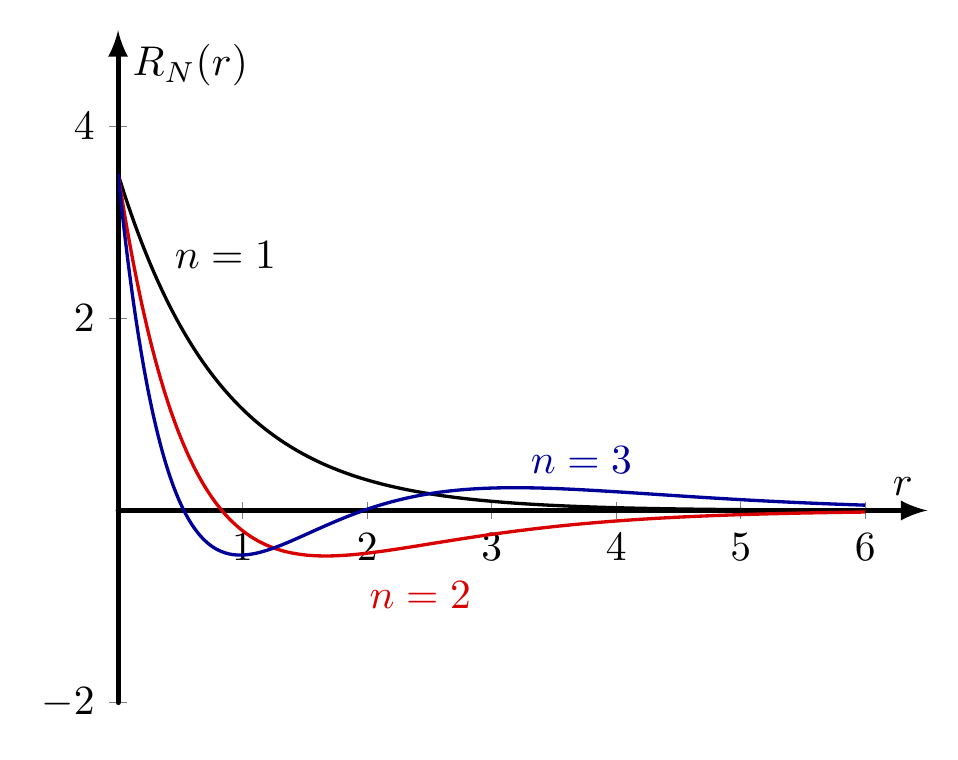
\begin{tikzpicture}[scale=1.5]
        \def\nu{1.2}
        \def\A{3.5}

        \begin{axis}[
            % Axis Setup
            axis lines = middle,
            axis line style = {-latex, very thick, line cap=round}, % Arrows and thick lines
            xlabel = {$r$},
            ylabel = {$R_N(r)$},
            xmin=0, xmax=6.5,
            ymin=-2, ymax=5,
        ]

        % --- Plot n=1 (Black) ---
        \addplot[
            domain=0:6, 
            samples=100, 
            smooth, 
            thick, 
            black
        ] 
        {\A * exp(-\nu * x)} 
        node[pos=0.15, above right, font=\bfseries] {$n=1$};

        % --- Plot n=2 (Red) ---
        \addplot[
            domain=0:6, 
            samples=100, 
            smooth, 
            thick, 
            red!85!black
        ] 
        {\A * (1 - \nu * x) * exp(-\nu * x)} 
        node[pos=0.6, below, font=\bfseries, yshift=-5pt] {$n=2$};

        % --- Plot n=3 (Blue) ---
        \addplot[
            domain=0:6, 
            samples=150, 
            smooth, 
            thick, 
            blue!60!black
        ] 
        {\A * (1 - 2*\nu * x + (2/3) * (\nu * x)^2) * exp(-\nu * x)} 
        node[pos=0.75, above, font=\bfseries, xshift=2pt] {$n=3$};

        \end{axis}
    \end{tikzpicture}
    \caption{Plot of Solutions to zero angular momentum problem}
    \label{figZeroLSolutions}
\end{figure}
\subsection{Solutions for Positive Angular Momentum}
Now our effective potential is different from our standard potential. Recall the TISE:
\begin{equation}
    -\frac{\hbar^2}{2m} \left(\frac{d^{2}R}{dr^{2}} + \frac{2}{r}\frac{dR}{dr}\right) + \left(U(r) + \frac{\hbar^2 l (l+1)}{2mr^2}\right) = ER(r)
    \tag{\ref{eqnHydrogenRadial}}
\end{equation}
We use a similar method. We have the same asymptotic behaviour as the $l = 0$ case, $R(r) \sim e^{-\nu r}$. We use the power series:
\begin{equation}
    g(r) = r^\sigma \sum_{n=0}^{\infty} a_n r^n
    \label{eqnPosLPowerSeries}
\end{equation}
Again we use the lowest power of $r$ to get the value of $\sigma$:
\begin{equation*}
    \sigma(\sigma + 1) = l(l+1) \implies \sigma \in \{-(l+1), l\}
\end{equation*}
We again discount the negative solution because it would give unphysical behaviour as $r \to 0$. Therefore, $\sigma = l$.
The recurrence relation for the coefficients of $g$ is:
\begin{equation}
    a_n = \frac{2\nu(n + l) - \beta}{n(n+2l-1)} a_{n-1}
    \label{eqnPosLPolyCoeffts}
\end{equation}
Then we require, as before, that $g$ is a polynomial. This requires a value $n_{\text{max}}$ such that $a_{n_{\text{max}}} = 0, a_{n_{\text{max}} - 1} \neq 0$.

This is when $2\nu (n_{\text{max}} + l) - \beta = 0$. We define $N = n_{\text{max}} + l$, in order to recover equation~\ref{eqnNuQuantisation}, the same as the case $l = 0$. We use the definition of $\nu$:
\begin{equation*}
    E_n = -\frac{e^4 m}{32\pi^2 \epsilon_0^2 \hbar^2} \frac{1}{N^2}
\end{equation*}
Therefore the eigenvalues are exactly the same as in the $l = 0$ case. However, the degeneracy is larger. For each $N = n_{\text{max}} + l$, we can have $N-1$ different values for $l$, and we also have $m_l \in [-l, l]$. The degeneracy is therefore:
\begin{equation*}
    D(N) = \sum_{l=0}^{N-1} \sum_{m=-l}^{l} 1 = N^2
\end{equation*}
So for each energy level $N$ we have $N^2$ different energy eigenfunctions. Putting this all together:
\begin{align*}
    \chi_{N, l, m}(r, \theta, \phi) &= R_{N, l}(r) Y_{l, m}(\theta, \phi) \\
    &= r^l g_{N, l}(r) e^{-\frac{\beta r}{2N}} Y_{l, m}(\theta, \phi)
\end{align*}
where $g$ is a polynomial of degree $N - l - 1$ defined by:
\begin{equation*}
    g_{N, l}(r) = \sum_{k=0}^{N- l - 1} a_{k}^{(N, l)}r^k
\end{equation*}
with coefficients given by:
\begin{equation*}
    a_{k}^{(N, l)} = \frac{2\nu}{k} \frac{k + l - N}{k + 2l + 1} a_{k - 1}^{(N, l)}.
\end{equation*}
These are the \underline{generalised Laguerre polynomials}.
\nonexaminablesubsection{Link to Chemistry}
In Chemistry, we have the $s$, $p$, and $d$ orbitals. We can show how these arise from different quantum numbers in the above equations.

The $1s$ orbital has $N = 1, l = 0$. It is given by the equation:
\begin{equation*}
    \chi_{1, 0, 0} = a_0^{(1, 0)} e^{-\frac{r\beta}{2}}
\end{equation*}
and this is a single spherical region of positive probability.

The $2s$ orbital has $N = 2, l = 0$. It is given by:
\begin{equation*}
    \chi_{2, 0, 0} = \left(a_0^{(2, 0)} + a_1^{(2, 0)}r\right) e^{-\frac{r\beta}{4}}
\end{equation*}
This has spherical symmetry, but the probability density is positive in a sphere around the origin, zero in disc around this, and then positive again in a larger disc before tending to 0.
% Find a good image to show this - perhaps the uploaded notes will contain one.

The $3s$ orbital how has 3 discs of positive probability, and this pattern continues.

The $1p$ orbital does not exist, because we impose $l < N$. The $2p$ orbital is given by:
\begin{align*}
    \chi_{2, 1, \pm 1} &= r a_0^{(2, 1)} e^{-\frac{r\beta}{3}} \sin(\theta) e^{\pm i \phi} \\
    \chi_{2, 1, 0} &= r a_0^{(2, 1)} e^{-\frac{r\beta}{3}} \cos(\theta)
\end{align*}
For the shapes of these, see figure~\ref{figOrbitals}.

We know have the required knowledge to critique the Bohr model of the Hydrogen atom.

Bohr correctly predicted the energy of each eigenstate, and the Bohr radius is proportional to the actual value - we found in Ex1Q6b that the actual value is $\frac32 a_0$.

However, the quantisation of angular momentum was incorrect. Bohr's model gives $L^2 = N^2 \hbar^2$, whereas we find that there are far more angular momentum values for each energy level, $L^2 = \hbar^2 l(l+1)$. Because of this, Bohr's predicted degeneracy of $N$ was incorrect, and we have shown that it is $N^2$.

To understand larger atoms, with more than one particle in the nucleus and more than one electron, we can consider a product of eigenfunctions for each electron, and the energy as the sum of the energies of each electron. However, this is a poor approximation because it does not account for the interactions between electrons and the exclusion principle (electrons cannot occupy the same eigenstate).
\end{document}